\newpage
\section{Auswertung}
\label{sec:Auswertung}
Im folgenden wird die Hysteresekurve des verwendeten Magneten bestimmt und aus der Verschiebung der Wellenlänge werden die Landé-Faktoren berechnet.



\subsection{Hysteresekurve}
In der Abbildung \eqref{fig:Hysterese} ist die Hysteresekurve des verwendeten Magneten zu sehen. Es ist eine Verschiebung der Kurve nach oben zu erkennen, allerdings sind mehrere Bereiche ohne Verschiebung dabei. Das kann durch die Ablesefehler des Feldstroms $I$ erklärt werden.
\begin{align*}
  \Delta I = 0.25\, \text{A}
\end{align*}
Die Ablesefehler kommen durch die analoge Anzeige zustande.

\begin{figure}[H]
  \centering
  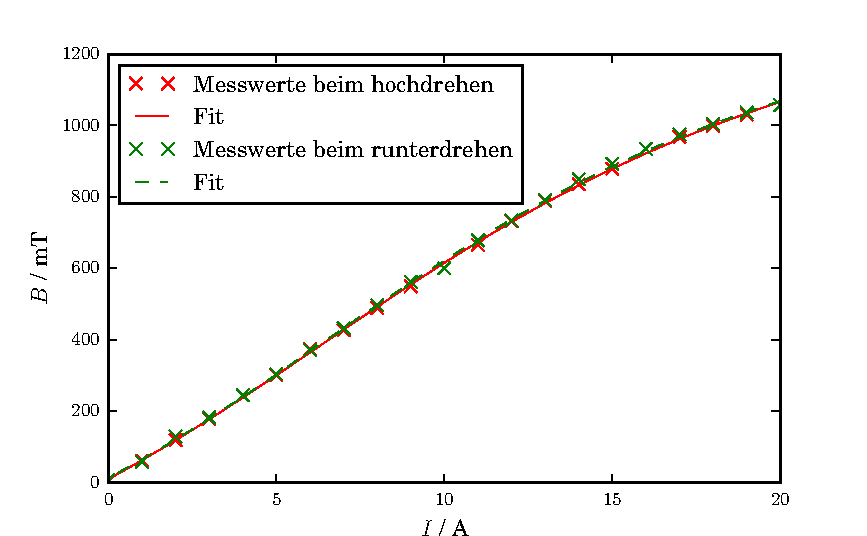
\includegraphics[width=\linewidth]{Bilder/Hysterese.pdf}
  \caption{Die Hysteresekurve des verwendeten Magneten.}
  \label{fig:Hysterese}
\end{figure}

Im folgenden wird der Fehler des B-Feldes auf 5\,\% geschätzt.


\subsection{Dispersionsgebiet}
Das Dispersionsgebiet gibt die maximale Wellenlängendifferenz an, die zwei Wellen haben dürfen ohne sich zu überlagern. Sie wird mit
\begin{align}
  \Delta\lambda_\text{D} = \frac{\lambda^2}{2\cdot d} \cdot \sqrt{\frac{1}{n^2 - 1}}
  \label{eqn:Dispersionsgebiet}
\end{align}
berechnet. $\lambda$ entspricht dabei der Wellenlänge der verwendeten Linie und $n$ der Brechzahl. Die Dicke der Lummer-Gehrcke Platte $d$ beträgt 4\,mm. Die Brechzahlen und Wellenlängen der roten und blauen Linie sind:
\begin{align*}
  \lambda_\text{rot} &= 643.8\,\text{nm} \\
  n_\text{rot} &= 1.4567 \\
  \lambda_\text{blau} &= 480.0\,\text{nm} \\
  n_\text{blau} &= 1.4635 \\
\end{align*}
Mit diesen Werten und der Formel \eqref{eqn:Dispersionsgebiet} ergeben sich folgende Dispersionsgebiete:
\begin{align*}
  \Delta\lambda_\text{D,rot} &= 0.0489 \cdot 10^{-9}\,\text{m}\ , \\
  \Delta\lambda_\text{D,blau} &= 0.0270 \cdot 10^{-9}\,\text{m}\ ,
\end{align*}
bestimmen.


\subsection{Wellenlängeänderung}
Die Wellenlängenänderung $\delta\lambda$ lässt sich mit
\begin{align}
  \delta\lambda = \frac{\delta\text{s}}{2\,\Delta\text{s}}\cdot \Delta\lambda_\text{D}
  \label{eqn:Verschiebung}
\end{align}
berechnen. $\Delta$s ist dabei der Abstand zwischen zwei Linien ohne ein äußeres B-Feld und $\delta$s ist der Abstand zwischen den aufgespaltenen Linien.



\subsubsection{Verschiebung der roten Linie}
\begin{figure}[H]
  \centering
  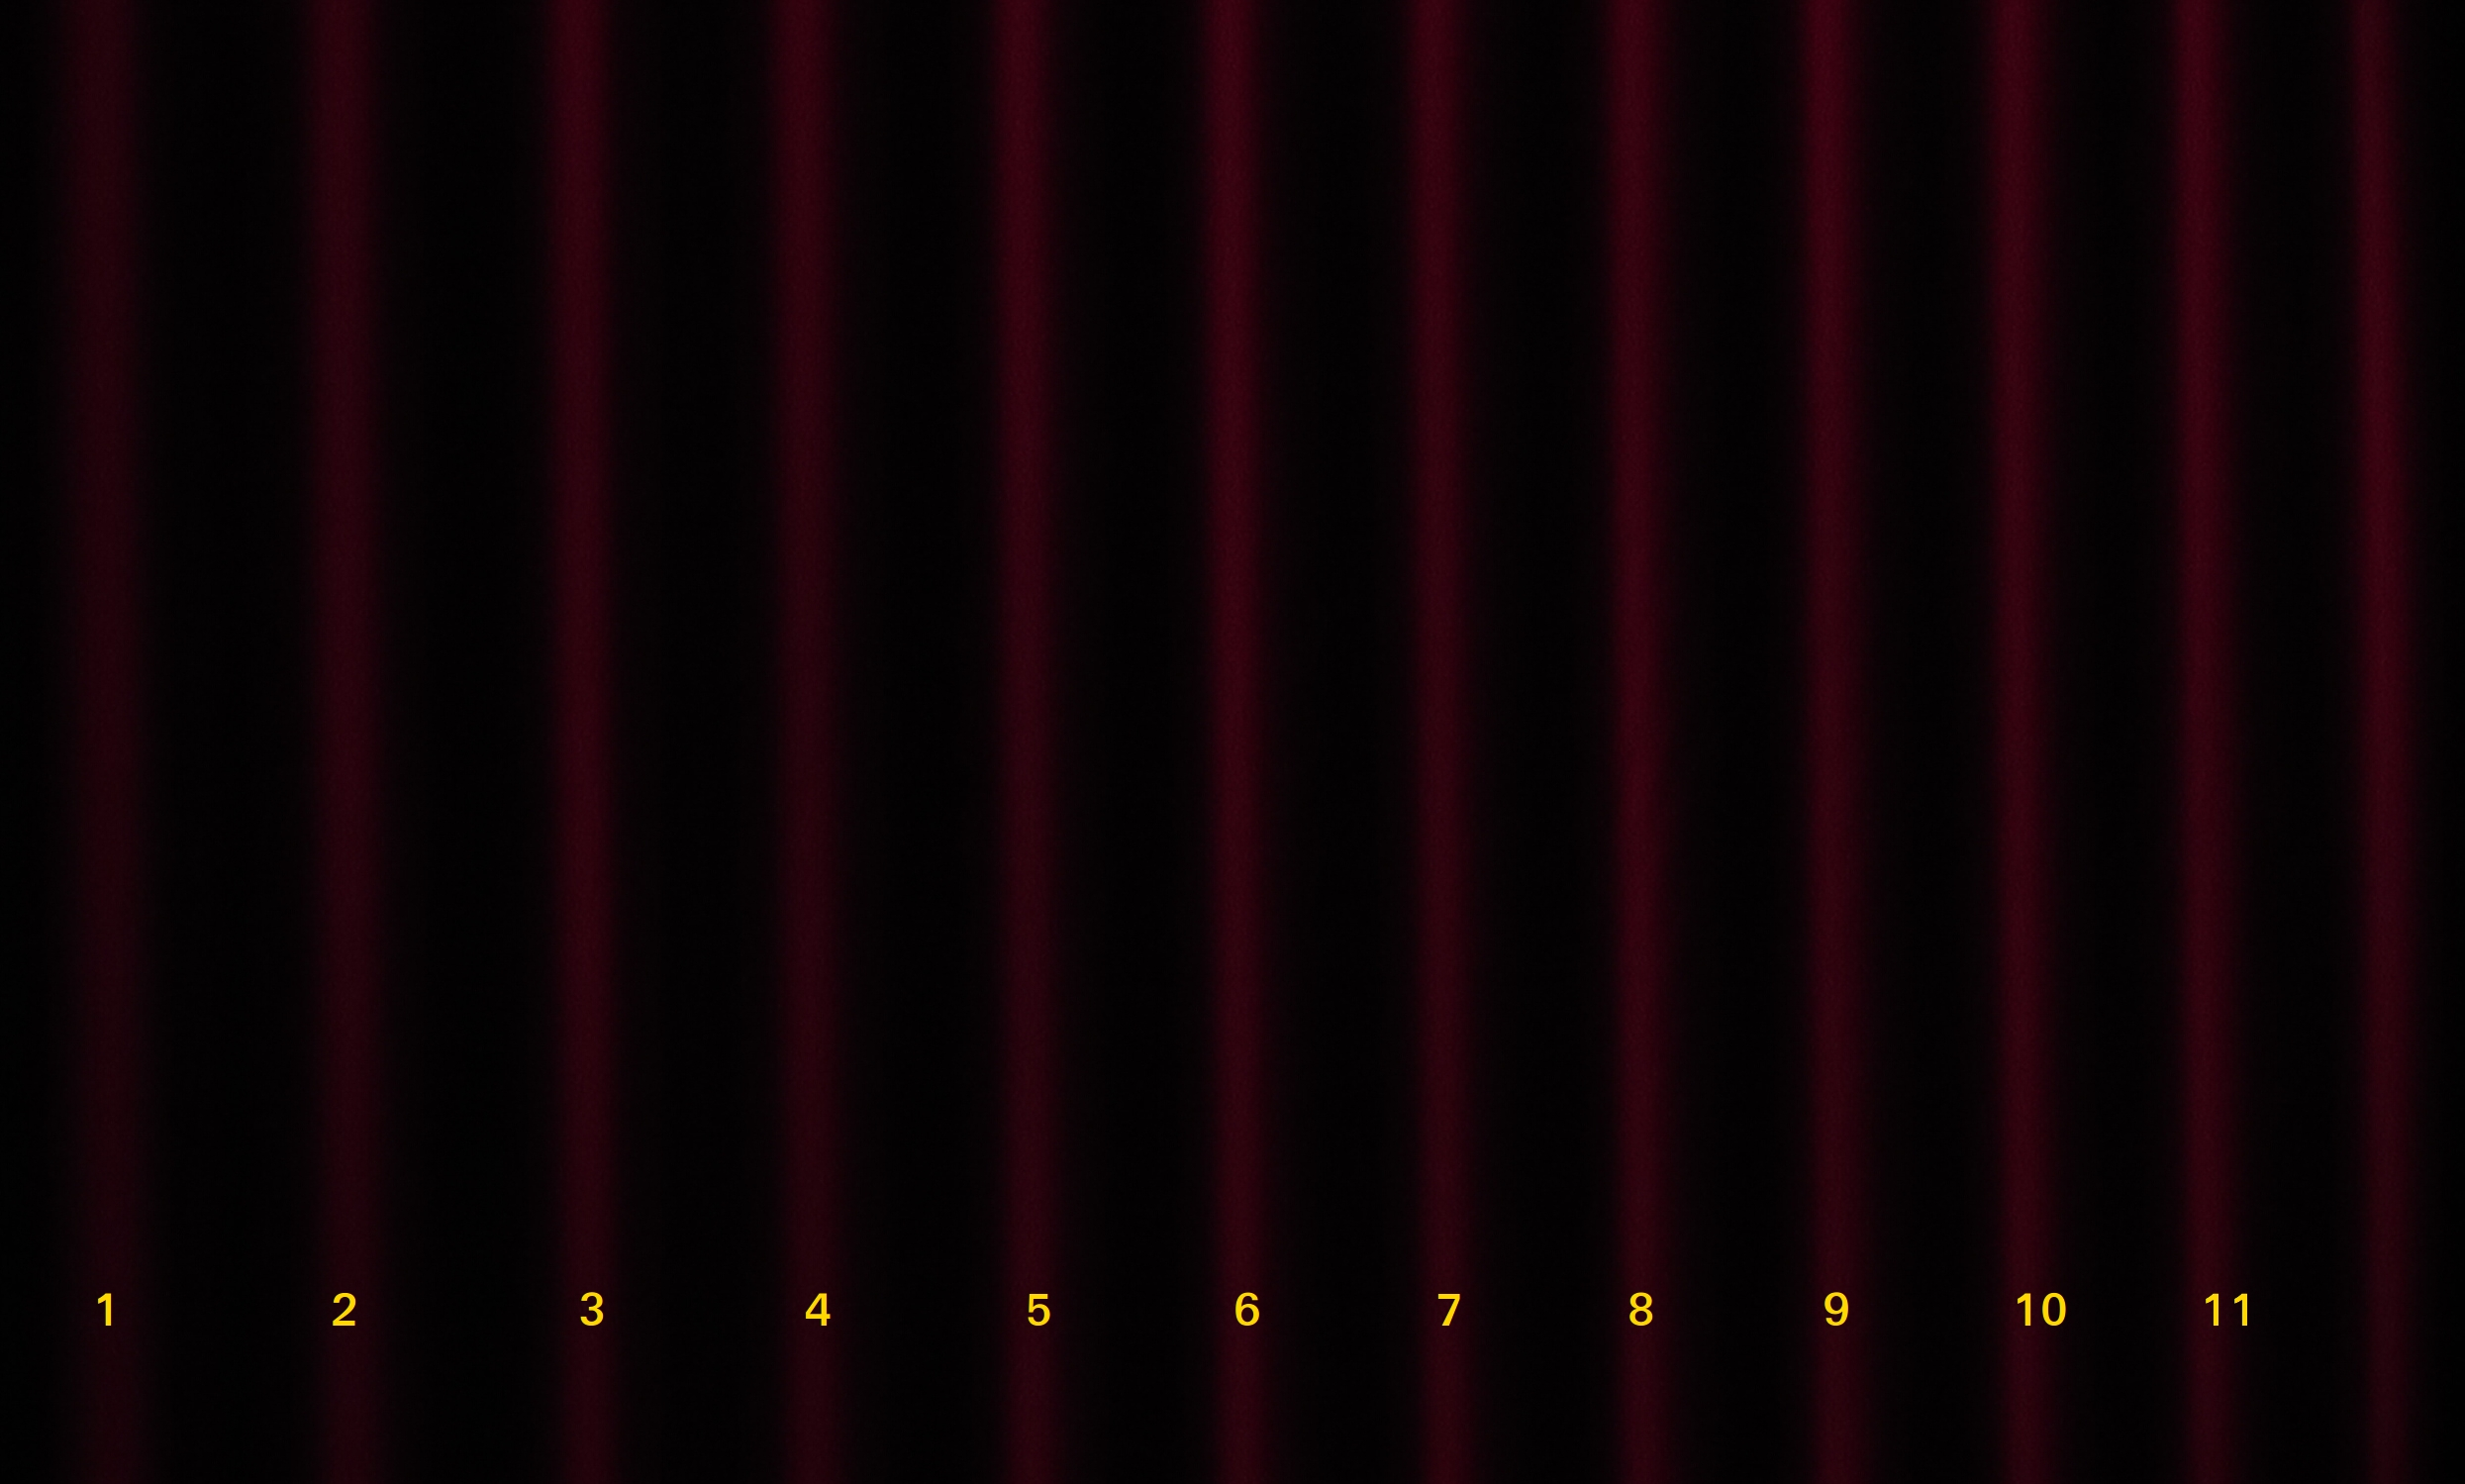
\includegraphics[width=0.8\linewidth]{Bilder/RoB.JPG}
  \caption{Die rote Linie der Cd-Lampe ohne ein äußeres B-Feld.}
  \label{fig:RoB}
\end{figure}

\begin{figure}[H]
  \centering
  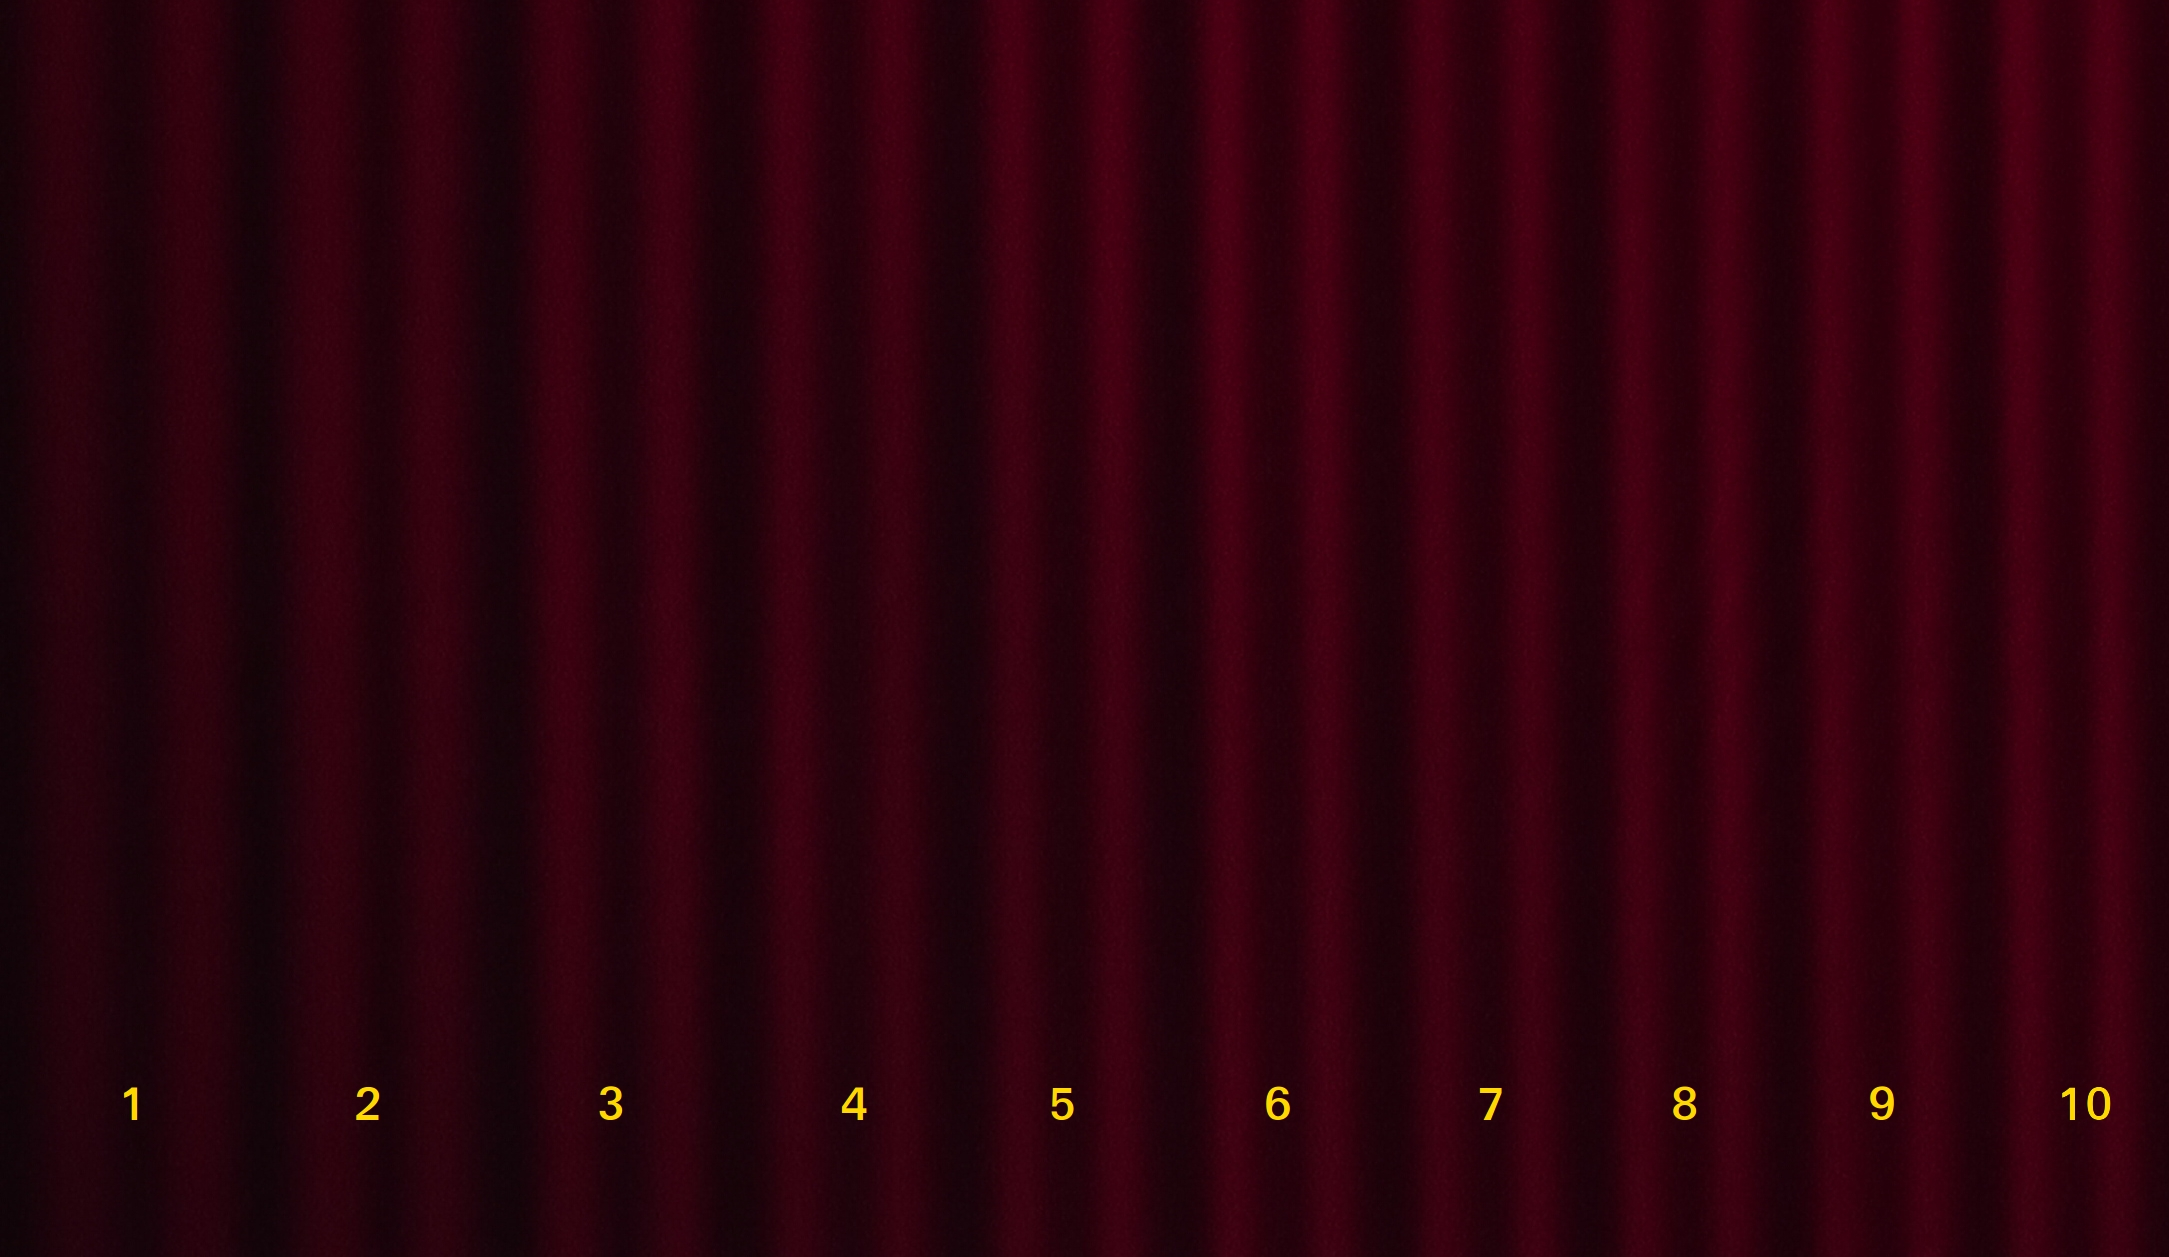
\includegraphics[width=0.8\linewidth]{Bilder/R9ASig.JPG}
  \caption{Die $\sigma$-Komponente der roten Linie der Cd-Lampe mit einem äußeren B-Feld ($B_{\sigma,\text{rot}} = (\num{0.55 +- 0.03})$\,T).}
  \label{fig:R9ASig}
\end{figure}

Die Werte für die Tabelle \eqref{tab:rot} werden aus den Abbildungen \eqref{fig:RoB} und \eqref{fig:R9ASig} bestimmt.

\begin{table}[H]
  \centering
  \caption{Messwerte für die Berechnung der Verschiebung der roten Linie.}
  \label{tab:rot}
  \begin{tabular}{c c c}
    $\Delta$s / Pixel & $\delta$s$_{\sigma}$ / Pixel & $\delta \lambda_{\sigma}$ / $10^{-12}$\,m \\
    \hline
    244.0 & 123.0 & 12.33 \\
    240.0 & 106.3 & 10.84 \\
    226.0 & 108.0 & 11.69 \\
    220.0 & 106.7 & 11.86 \\
    213.0 & 101.3 & 11.63 \\
    206.0 & 95.7  & 11.36 \\
    201.0 & 97.7  & 11.88 \\
    193.0 & 93.0  & 11.78 \\
    188.0 & 91.0  & 11.84 \\
    191.0 & 84.7  & 10.84 \\
    \hline
  \end{tabular}
\end{table}

Mit Hilfe der Formel \eqref{eqn:Verschiebung}, der Dispersionsgebiete und der Tabelle \eqref{tab:rot} ergeben sich nach dem mitteln folgende Werte für die Verschiebung $\delta\lambda$:
\begin{align*}
  \delta \lambda_{\sigma,\text{rot}} = (\num{11.6 +- 0.4})\cdot 10^{-12}\,\text{m} \\
\end{align*}



\subsubsection{Verschiebung der blauen Linie}
\begin{figure}[H]
  \centering
  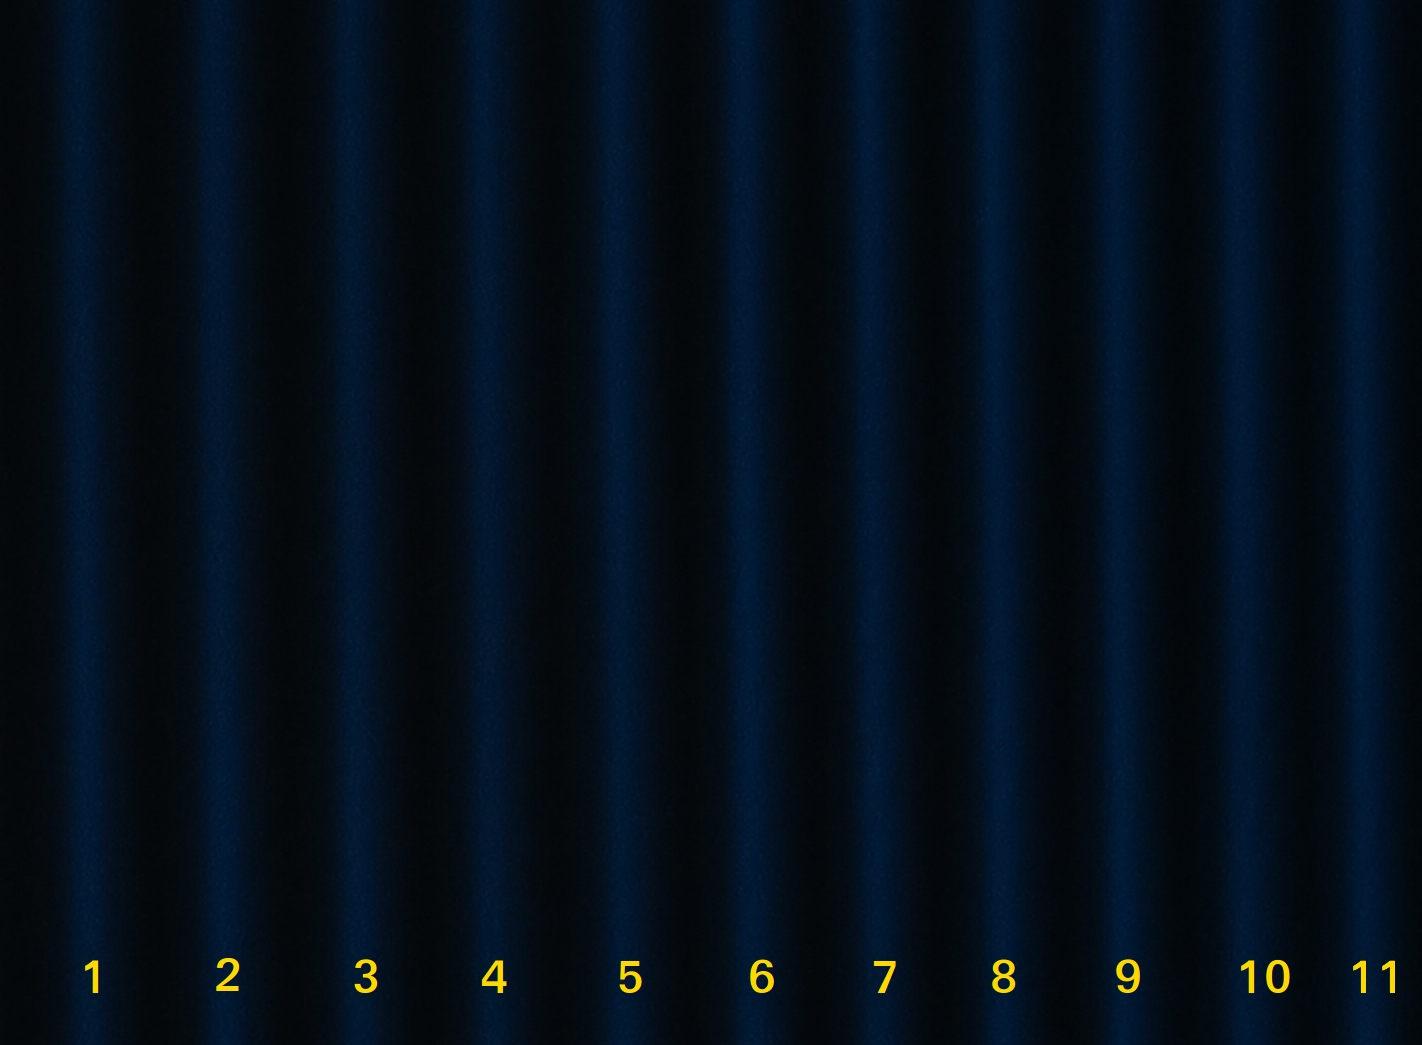
\includegraphics[width=0.8\linewidth]{Bilder/BoB.JPG}
  \caption{Die blaue Linie der Cd-Lampe ohne ein äußeres B-Feld.}
  \label{fig:BoB}
\end{figure}

\begin{figure}[H]
  \centering
  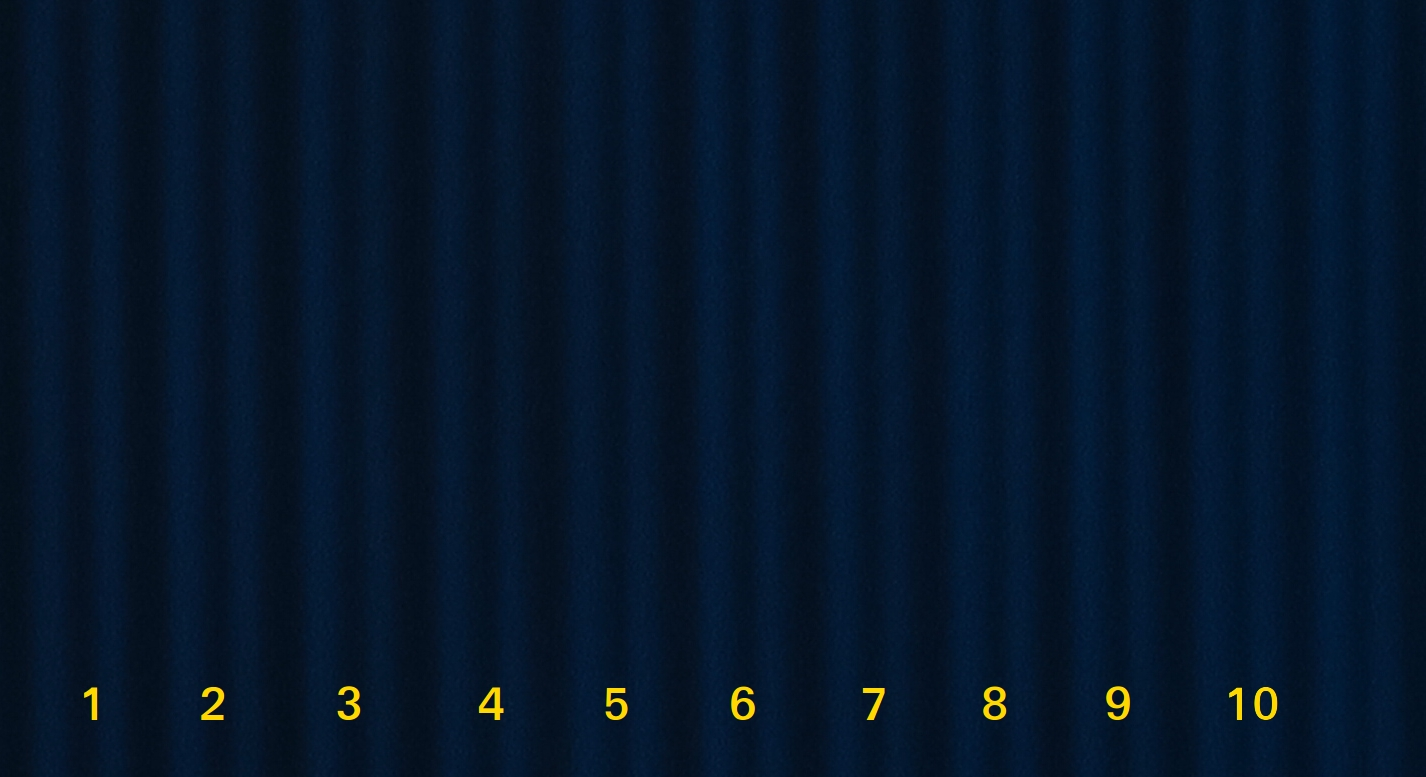
\includegraphics[width=0.8\linewidth]{Bilder/B6ASig.JPG}
  \caption{Die $\sigma$-Komponente der blauen Linie der Cd-Lampe mit einem äußeren B-Feld ($B_{\sigma,\text{blau}} = (\num{0.30 +- 0.02})$\,T).}
  \label{fig:B6ASig}
\end{figure}

\begin{figure}[H]
  \centering
  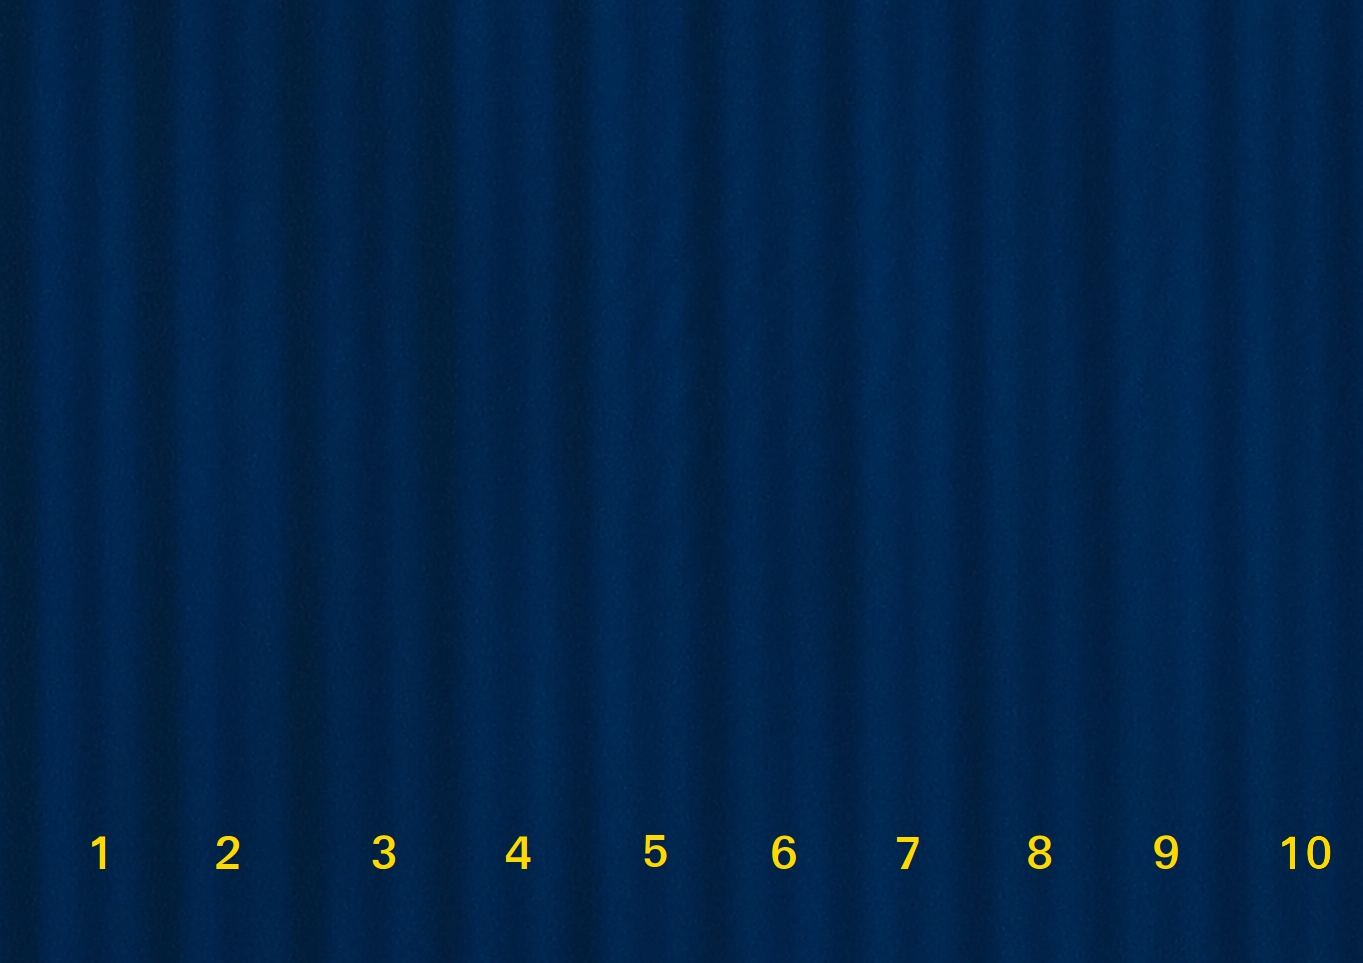
\includegraphics[width=0.8\linewidth]{Bilder/B20APi.JPG}
  \caption{Die $\pi$-Komponente der blauen Linie der Cd-Lampe mit einem äußeren B-Feld ($B_{\pi,\text{blau}} = (\num{1.06 +- 0.05})$\,T).}
  \label{fig:B20APi}
\end{figure}

Die Werte für die Tabelle \eqref{tab:blau} werden aus den Abbildungen \eqref{fig:BoB} bis \eqref{fig:B20APi} bestimmt.

\begin{table}[H]
  \centering
  \caption{Messwerte für die Berechnung der Verschiebung der blauen Linie.}
  \label{tab:blau}
  \begin{tabular}{c | c c | c c}
    $\Delta$s / Pixel & $\delta$s$_{\sigma}$ / Pixel & $\delta \lambda_{\sigma}$ / $10^{-12}$\,m & $\delta$s$_{\pi}$ / Pixel & $\delta \lambda_{\pi}$ / $10^{-12}$\,m \\
    \hline
    132.7 & 62.7 & 6.37 & 62.0 & 12.33 \\
    135.3 & 56.0 & 5.58 & 65.3 & 10.84 \\
    134.0 & 57.3 & 5.77 & 66.0 & 11.69 \\
    128.7 & 58.7 & 6.14 & 65.3 & 11.86 \\
    130.7 & 55.3 & 5.71 & 61.3 & 11.63 \\
    124.7 & 54.0 & 5.84 & 63.3 & 11.36 \\
    123.3 & 55.3 & 6.05 & 54.0 & 11.88 \\
    122.0 & 52.0 & 5.74 & 57.3 & 11.78 \\
    122.0 & 51.3 & 5.67 & 56.0 & 11.84 \\
    122.0 & 54.7 & 6.04 & 54.0 & 10.84 \\
    \hline
  \end{tabular}
\end{table}


Mit Hilfe der Formel \eqref{eqn:Verschiebung}, der Dispersionsgebiete und der Tabelle \eqref{tab:blau} ergeben sich nach dem mitteln folgende Werte für die Verschiebung $\delta\lambda$\,:
\begin{align*}
  \delta \lambda_{\sigma,blau} = (\num{5.9 +- 0.2})\cdot 10^{-12}\,\text{m} \\
  \delta \lambda_{\pi,blau} = (\num{6.4 +- 0.3})\cdot 10^{-12}\,\text{m}
\end{align*}



\subsection{Landé-Faktoren}
Die Landé-Faktoren $g_\text{ij}$ können nach umstellen der Formel \eqref{eqn:dE} bestimmt werden.
\begin{align}
  g_{ij} = m_1\,g_1 + m_2\,g_2 = \frac{\Delta E}{\mu_\text{B}\,B}
\end{align}
Dabei ist das Bohrsche Magneton gegeben durch $\mu_\text{B} = 9.274 \cdot 10^{-24}\,\frac{\text{J}}{\text{T}}$.\\
Die Energiedifferenz kann über
\begin{align}
  |\Delta E| \approx \left| \frac{\partial E}{\partial \lambda}\right| \cdot |\delta\lambda| = \frac{h\,c}{\lambda^2}\cdot \delta\lambda
\end{align}
berechnet werden. Dabei ist eingegangen, dass sich $\Delta E$ nicht linear mit $\lambda$ ändert. Damit ergibt sich für die Landé-Faktoren $g_{ij}$:
\begin{align}
  g_{ij} = \frac{h\,c}{\mu_\text{B}}\,\frac{\delta\lambda}{B\,\lambda^2}
  \label{eqn:Landé}
\end{align}



\subsubsection{Landé-Faktoren der roten Linie}
Der theoretische Landé-Faktor der roten Linie ist gleich 1 ($g_\text{theo,rot} = 1$), weil die Gesamtspinquantenzahl gleich 0 ist ($S$ = 0). \\
Das B-Feld für die Messung beträgt
\begin{align*}
  B_{\sigma,\text{rot}} = \num{0.55 +- 0.03} \text{T} \ .
\end{align*}
Der experimentelle Landé-Faktor wird mit Formel \eqref{eqn:Landé} zu
\begin{align*}
  g_{\text{exp},\sigma,\text{rot}} = \frac{h\,c}{\mu_\text{B}}\,\frac{\delta \lambda_{\sigma,\text{rot}}}{B_{\sigma,\text{rot}}\,\lambda_\text{rot}^2} = \num{1.09 +- 0.07}
\end{align*}
berechnet.


\subsubsection{Landé-Faktoren der blauen Linie}
Die theoretischen Landé-Faktoren der blauen Linie kann mit Formel \eqref{eqn:Lan} bestimmt werden. Damit ergibt sich ein Landé-Faktor der $\pi$-Komponente $g_{\text{theo},\pi,\text{blau}} = 0.5$. Für die $\sigma$-Komponente ergeben sich $g_{\text{theo},\sigma,\text{blau},1} = 1.5$ und $g_{\text{theo},\sigma,\text{blau},2} = 2.0$. Allerdings kann wegen der geringen Abweichung nur eine Linie erkannt werden. Deswegen wird der Landé-Faktor zu $g_{\text{theo},\sigma,\text{blau}} = 1.75$ gemittelt.
Das B-Feld für die Messungen beträgt
\begin{align*}
  B_{\sigma,\text{blau}} = \num{0.3 +- 0.02}\, \text{T}\ , \\
  B_{\pi,\text{blau}} = \num{1.06 +- 0.05}\, \text{T}\ .
\end{align*}
Die experimentellen Landé-Faktoren werden zu
\begin{align*}
  g_{\text{exp},\sigma,\text{blau}} &= \frac{h\,c}{\mu_\text{B}}\,\frac{\delta \lambda_{\sigma,\text{blau}}}{B_{\sigma,\text{blau}}\,\lambda_\text{blau}^2} = \num{1.8 +- 0.1} \\
  g_{\text{exp},\pi,\text{blau}} &= \frac{h\,c}{\mu_\text{B}}\,\frac{\delta \lambda_{\pi,\text{blau}}}{B_{\pi,\text{blau}}\,\lambda_\text{blau}^2} = \num{0.56 +- 0.04}
\end{align*}
bestimmt.





















%
